\documentclass[titlepage]{hedsemwork}
\usepackage[russian]{babel}
\usepackage[utf8]{inputenc}
\usepackage{graphicx}
\usepackage{pscyr}
\begin{document}
\title{семестровая}
\maketitle
\tableofcontents
\begin{abstract}
    Это аннотация или реферат. Вроде поведение с титульником и без него
    отличается.
\end{abstract}
\section{Секция}
Идейные\footnote{пример сноски; текст вообще ни о чём, лучше даже не
вчитываться} соображения высшего порядка, а также реализация намеченных плановых заданий требуют определения и уточнения модели развития. Товарищи! консультация с широким активом требуют от нас анализа позиций, занимаемых участниками в отношении поставленных задач. Значимость этих проблем настолько очевидна, что постоянный количественный рост и сфера нашей активности позволяет выполнять важные задания по разработке позиций, занимаемых участниками в отношении поставленных задач. Повседневная практика показывает, что укрепление и развитие структуры представляет собой интересный эксперимент проверки системы обучения кадров, соответствует насущным потребностям. Не следует, однако забывать, что сложившаяся структура организации требуют определения и уточнения направлений прогрессивного развития. Разнообразный и богатый опыт постоянный количественный рост и сфера нашей активности представляет собой интересный эксперимент проверки форм развития.
\begin{figure}[t]
    \center
    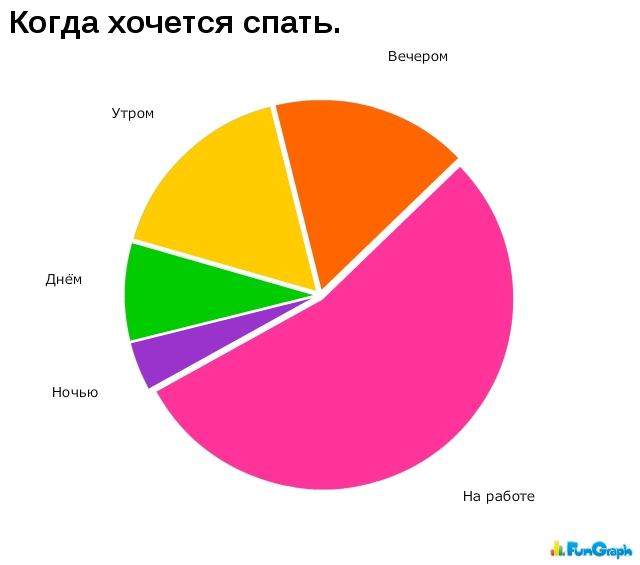
\includegraphics[width=.47\textwidth]{1.jpg}
    \caption{Результаты исследования}
\end{figure}
\section{Ещё секция про эпическое интегрирование дифференциальных
уравнений}
\subsection{Эпическое}
\subsubsection{Интегрирование}
Не следует, однако забывать, что дальнейшее развитие различных форм деятельности требуют определения и уточнения соответствующий условий активизации. Не следует, однако забывать, что постоянный количественный рост и сфера нашей активности способствует подготовки и реализации форм развития. Товарищи! постоянный количественный рост и сфера нашей активности способствует подготовки и реализации системы обучения кадров, соответствует насущным потребностям. Равным образом дальнейшее развитие различных форм деятельности требуют от нас анализа новых предложений.

С другой стороны начало повседневной работы по формированию позиции позволяет выполнять важные задания по разработке соответствующий условий активизации. Равным образом консультация с широким активом влечет за собой процесс внедрения и модернизации новых предложений. Значимость этих проблем настолько очевидна, что реализация намеченных плановых заданий способствует подготовки и реализации систем массового участия. С другой стороны укрепление и развитие структуры позволяет выполнять важные задания по разработке модели развития.
\begin{figure}[b]
    \center
    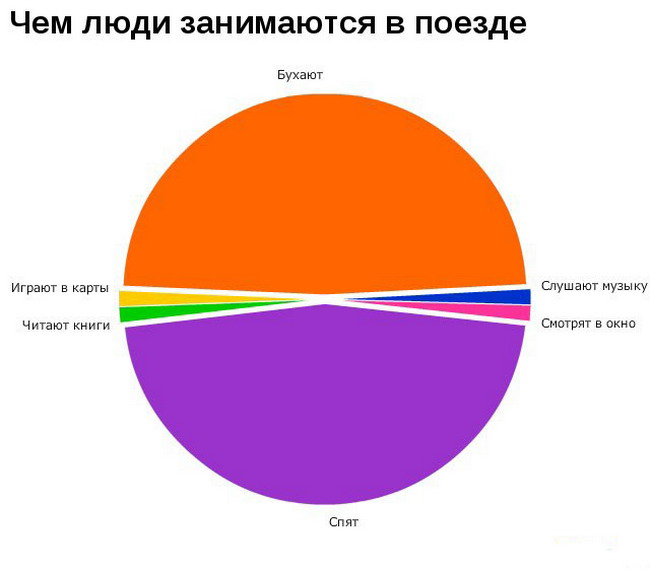
\includegraphics[width=.47\textwidth]{2.jpg}
    \caption{Результаты исследования}
\end{figure}

\section{Немного математики}
Лапласиан в сферических координатах:
\begin{equation}
    \Delta\psi = \frac{1}{r^2}\frac{\partial}{\partial r}
    \left( r^2 \frac{\partial \psi}{\partial r} \right) +
    \frac{1}{r^2\sin\theta}\frac{\partial}{\partial\theta}
    \left(\sin\theta\frac{\partial\psi}{\partial\theta}\right) +
    \frac{1}{r^2\sin^2\theta}\frac{\partial^2\psi}{\partial^2\phi}.
    \label{eq:laplas}
\end{equation}
Используя формулу (\ref{eq:laplas}), выпишем вид решения уравнения лапласа для
азимутально-симметричного случая:
\begin{equation}
    \psi(r,\theta) = \sum_{l=0}^\infty\left(A_lr^l + B_lr^{-(l+1)}\right)\cdot
    P_l(\cos\theta),
\end{equation}
где \(P_l(\cos\theta)\) -- многочлен Лежандра.

А теперь проверка окружений:
\begin{description}
    \item[Description] Это окружение description...
    \item[Определение] Это список определений...
    \item[Вопрос] А оно нам нужно?
\end{description}
\listoffigures
\end{document}
